\documentclass[12pt]{article}

\usepackage[utf8]{inputenc}
\usepackage{graphicx}
\usepackage{fancyhdr}
\usepackage{float}

\title{\textit{g55\_system} - Crazy Eights Card Game}
\author{Group 55\\Juliette Regimbal (260657238)\\Qingzhou Yang (260687570)}
\date{April 11, 2017}
\pagenumbering{gobble}
\pagenumbering{arabic}
\pagestyle{fancy}

\begin{document}
\maketitle
\setlength{\parindent}{0ex}
\lhead{Group 55}
\rhead{Juliette Regimbal (260657238)\\Qingzhou Yang (260687570)}

\section{Description and User Operation}
The circuit \textit{g55\_system} refers to the complete circuit designed to simulate a game of Crazy Eights with a computer player. Both the player and computer should received 7 random cards from a standard 52 card deck. Each then takes turns either playing a legal card on top of the play pile (where the first card is randomly chosen from the deck) or drawing a card from the deck. The entire system has 4 1-bit inputs (\texttt{clock}, \texttt{reset}, \texttt{play\_req\_sel}, and \texttt{make\_move\_raw}),  1 6-bit input (\texttt{card\_sel}), 4 7-bit outputs (seven segment displays named \texttt{ss\_td\_val}, \texttt{ss\_td\_suit}, \texttt{ss\_pd\_val}, and \texttt{ss\_pd\_suit}), 1 2-bit output (\texttt{win\_out}), 1 6-bit output (\texttt{player\_num}), and 1 1-bit output (\texttt{player\_legal}).  These inputs and outputs inform the user about the status of the game and cards currently in their possession, and also allows for the player to either play or draw a card on their turn. Explanations for each input and output are as follows:\\

\begin{enumerate}
\item \textbf{Inputs}
\begin{itemize}
\item \texttt{clock} - 1-bit input connected to a 50MHz clock pulse produced by the FPGA.
\item \texttt{reset} - asynchronous reset mapped to the push button KEY0.
\item \texttt{play\_req\_sel} - selects the action the player wishes to make; 0 signals the player will play the selected card (if legal) and 1 signals the player will draw a card from the deck. It is mapped to SW0.
\item \texttt{make\_move\_raw} - signals all other inputs are set properly and the player is ready to make their move; mapped to push button KEY3.
\item \texttt{card\_sel} - selects the number of card in the player's possession to play, displaying the suit on HEX1 and the value on HEX0. The number is a binary unsigned integer and mapped on SW9 down to SW4 where SW9 is the MSB.
\end{itemize}
\item \textbf{Outputs}
\begin{itemize}
\item \texttt{ss\_td\_val} - the value of the top card on the play pile mapped to HEX2.
\item \texttt{ss\_td\_suit} - the suit of the top card on the play pile mapped to HEX3.
\item \texttt{ss\_pd\_val} - the value of the currently selected card in the player's hand mapped to HEX0.
\item \texttt{ss\_pd\_suit} - the suit of the currently selected card in the player's hand mapped to HEX1.
\item \texttt{player\_num} - the number of cards in the player's hand represented in binary. It is mapped to LEDR5 down to LEDR0 where LEDR5 is the MSB.
\item \texttt{player\_legal} - 1 if the currently selected card can be legally played, 0 otherwise. It is mapped to LEDG7.
\item \texttt{win\_out} - 00 if the game is ongoing, 10 if the player has won, and 01 if the computer has won. The MSB is mapped to LEDG0 and the LSB is mapped to LEDR9.
\end{itemize}
\end{enumerate}

\section{Circuit Design}
\begin{figure}[H]
\centering
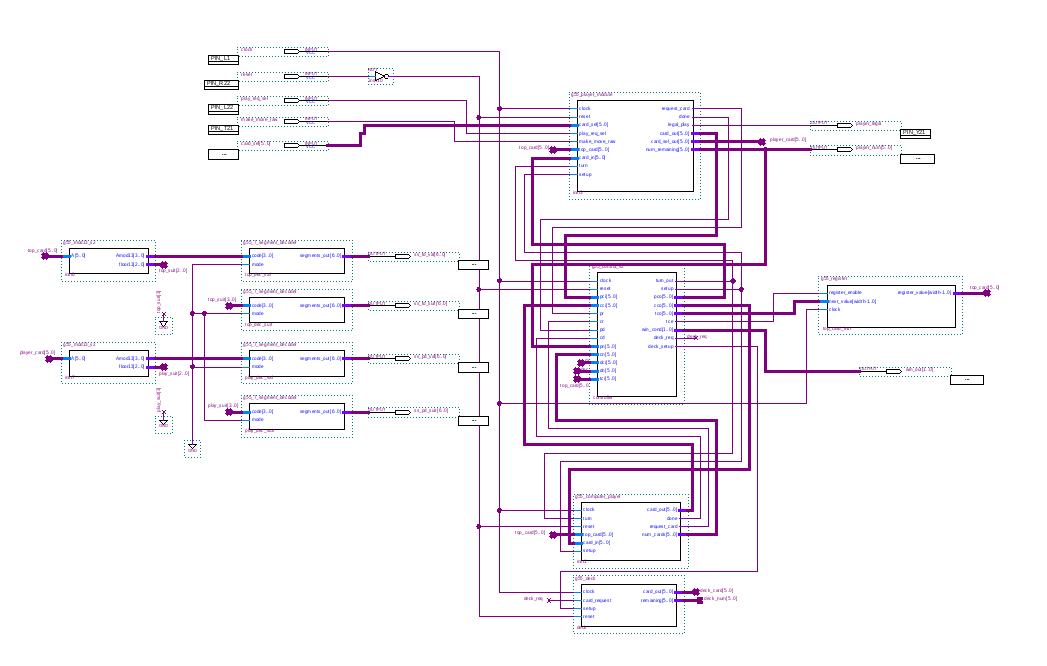
\includegraphics[scale = 0.45, angle=90, origin=c]{graphics/complete-circuit.png}
\caption{\textit{g55\_system\_v2} Schematic}
\end{figure}

\begin{figure}[H]
\centering
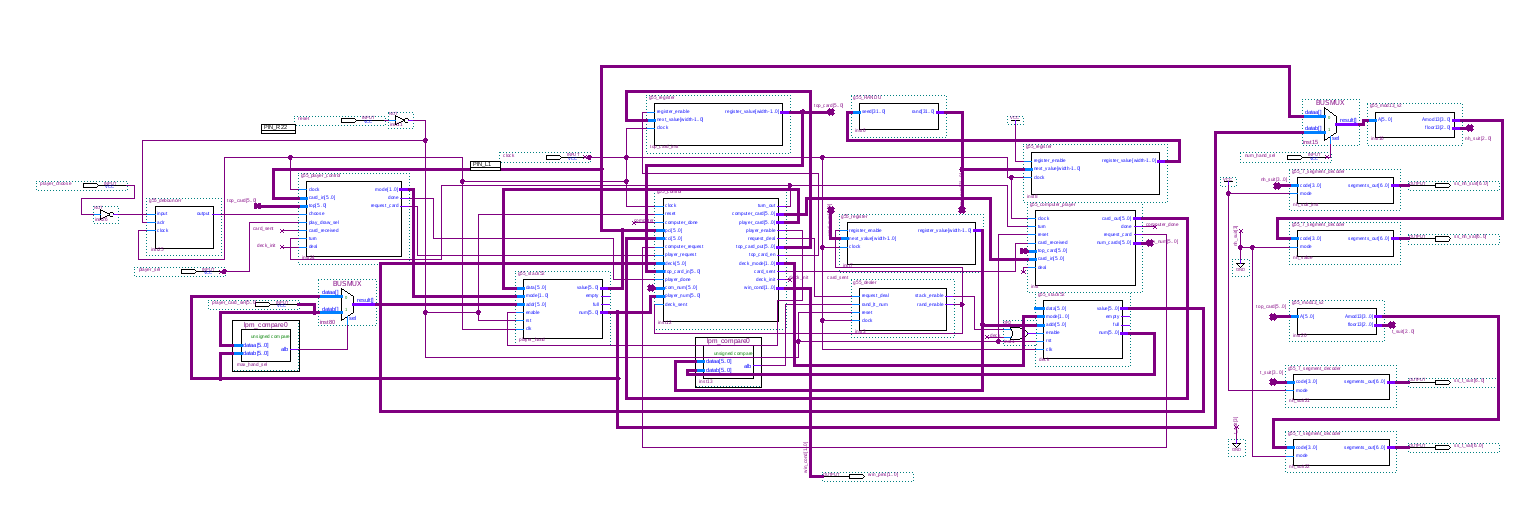
\includegraphics[scale=0.3, angle = 90, origin = c]{graphics/initial-circuit.png}
\caption{\textit{g55\_system} Schematic}
\end{figure}

Two versions of the circuit were made: an initial attempt (\textit{g55\_system} in Figure 2) and a second attempt (\textit{g55\_system\_v2} in Figure 1). In all other sections, \textit{g55\_system} refers to \textit{g55\_system\_v2}, not the first version. The first version is included solely as a record, and is not the subject of discussion in this section. The circuit is composed of three main modules: the player module, the computer player module, and the controller. The player module and computer player module handle the moves made and cards possessed by the player and computer player respectively. They are directed by the controller, which keeps track of whose turn it is and if the game has been won. The controller also updates the card on the top of the play pile, which is represented by a 6-bit register that is updated with the encoded value of each played card. Previous valules do not affect gameplay and are discarded. The controller is able to request cards directly from the deck, which is composed of a stack (\textit{g55\_stack52}), a dealer that ensures it is getting a valid card from the stack (\textit{g55\_dealer}), and a pseudorandom number generator that chooses an address in the stack (\textit{g55\_rand\_sync}, which is a synchronous implementation of the \textit{g55\_RANDU} circuit).\\

The circuit also contains four seven segment displays, that allow the user to see the card selected from their hand and the current card on top of the play pile. To decode the encoded cards to a readable form, two modulo 13 circuits (\textit{g55\_mod13\_v2}) are used.

\subsection{Player Module}

The player module (\textit{g55\_player\_module}) is a finite state machine (FSM) that contains a stack (\textit{g55\_stack52}), a rules checker (\textit{g55\_rules}), a debouncer (\textit{g55\_debouncer}), a 6-bit muxer (\textit{busmux}), and a 6-bit less than comparator (\textit{lpm\_compare0}). The stack contains the cards in the player's hand. The debouncer takes the input \texttt{make\_move\_raw} and removes the noise so it produces a single pulse. The rules module ensures the selected card in the stack is legal to play with the current top play pile card. The muxer and comparator are present to ensure that the player does not input an address in the stack that is greater than the number of entries, returning the highest address with an entry in the case where the specified address is too high. \\

The FSM begins in a wait state waiting for the controller to signal that it is now the player's turn (\texttt{turn} = 0). At that point, it transitions to the next state where it waits for the \texttt{make\_move} input to go to 1. At that point, it will either request a card from the controller (draw a card from the deck), or it will send a card to the controller and end its turn by asserting the \texttt{done} signal. When requesting a card, the \texttt{request\_card} signal is asserted and the module waits on the input \texttt{card\_in} to change, assuming that when it changes that new value is the requested card. If the controller asserts the \texttt{setup} signal, the FSM will go immediately to request a card. This is used to deal the initial cards to the player. The inputs and outputs are as follows:\\

\begin{enumerate}
\item Inputs
\begin{itemize}
\item \texttt{clock} - clock input for the circuit.
\item \texttt{reset} - asynchronous reset signal.
\item \texttt{card\_sel} - 6-bit input specifying the address in the stack of a card.
\item \texttt{play\_req\_sel} - the 1-bit input selecting the operation as specified in section 1.
\item \texttt{make\_move\_raw} - the raw signal confirming the selected move.
\item \texttt{top\_card} - the 6-bit encoded card currently on top of the play pile.
\item \texttt{card\_in} - the 6-bit encoded card input sent to the module by the controller.
\item \texttt{turn} - the signal specifying if it is the computer's turn (1) or the player's (0).
\item \texttt{setup} - the signal specifying if the game is being set up and if the module should accept dealt cards.
\end{itemize}
\item Outputs
\begin{itemize}
\item \texttt{request\_card} - the signal sent to the controller that shows the user wants to draw a card from the deck.
\item \texttt{done} - the signal asserted to mark the end of the player's turn.
\item \texttt{legal\_play} - the signal asserted when the card selected in the stack is a legal move given the top card on the play pile.
\item \texttt{card\_out} - 6-bit output to send a card to the controller.
\item \texttt{card\_sel\_out} - the 6-bit encoded card currently selected in the stack.
\item \texttt{num\_remaining} - the number of cards remaining in the user's hand (the stack).
\end{itemize}
\end{enumerate}  

\subsection{Computer Player Module}
The computer player circuit (\textit{g55\_computer\_player}) is the other player in the game. It is a FSM that waits for the controller to signal its turn, goes through all the cards in its hand, and if a card that is legal to play is found it plays that. Otherwise, it draws a card from the deck.  The circuit implements a stack (\textit{g55\_stack52}) and a rules checker (\textit{g55\_rules}). It follows the same communication protocol with the controller as the player module. The inpupts and outputs are as follows:\\

\begin{enumerate}
\item Inputs
\begin{itemize}
\item \texttt{clock} - clock input for the circuit.
\item \texttt{reset} - asynchronous reset signal.
\item \texttt{turn} - the signal specifying if it is the computer's turn (1) or the player's (0).
\item \texttt{top\_card} - the 6-bit encoded card currently on top of the play pile.
\item \texttt{card\_in} - the 6-bit encoded card being sent to the module by the controller.
\item \texttt{setup} - the signal specifying if the game is being set up and if the module should accept dealt cards.
\end{itemize}
\item Outputs
\begin{itemize}
\item \texttt{card\_out} - 6-bit output to send a card to the controller.
\item \texttt{done} - the signal asserted to mark the end of the computer player's turn.
\item \texttt{request\_card} - the signal sent to the controller that shows the computer player wants to draw a card from the deck.
\item \texttt{num\_cards} - the number of cards remaining in the computer player's hand (the stack).
\end{itemize}
\end{enumerate}

\subsection{Controller}
The controller circuit (\textit{g55\_control\_v2}) is a FSM that directs gameplay. It begins in a setup state where it signals the deck stack to initialize back to its full 52 card state. After this it requests a card from the deck and sends it to the player and then to the computer player, repeating this until each has 7 unique cards. Then finally it requests a last card that is used as the initial top card. Frorm here it begins typical gameplay.\\

In typical gameplay, first the controller inverts the \texttt{turn} signal from one player to the other, and then checks if the conditions for a game to be won (either player having no cards) have been met. If this is the case, it updates \texttt{win\_cond} as specified in section 1 and then transitions to the game over state. It will remain in a game over state until the asynchronous reset signal is asserted by the user. Otherwise, it waits for the current player to either assert the \texttt{done} signal or the \texttt{request\_card} signal. There are separate inputs for the computer player and human player. If the done signal is asserted, the controller takes the input sent to it and makes it the new top card. It then returns to the check state. If the card request signal is asserted, then the controller forwards that request to the deck and waits to receive a card. When it does, it sends this card to the player who requested it, and waits for that player to assert the done signal. Then it transitions back to the check state. In order to check when a value has been received, it stores the last received value for each 6-bit encoded card input from the player, computer, top card, and the deck. When these values change, it signals the controller it has receivevd the value it was waiting on (assuming it was waiting on any signal). The inputs and outputs are as follows:\\

\begin{enumerate}
\item Inputs
\begin{itemize}
\item \texttt{clock} - clock input for the circuit.
\item \texttt{reset} - asynchronous reset signal.
\item \texttt{pci} - player card input; the 6-bit encoded card input sent by the player.
\item \texttt{cci} - computer card input; the 6-bit encoded card input sent by the computer.
\item \texttt{pr} - player request; the signal asserted by the player when it requests a card from the deck.
\item \texttt{cr} - computer request; the signal asserted by the computer when it requests a card from the deck.
\item \texttt{pd} - player done; the signal asserted by the player when their turn is completed.
\item \texttt{cd} - computer done; the signal asserted by the computer when its turn is completed.
\item \texttt{pn} - player number; the 6-bit number representing the number of cards in the player's hand.
\item \texttt{cn} - computer number; the 6-bit number representing the number of cards in the computer's hand.
\item \texttt{dci} - deck card input; the 6-bit encoded card input sent by the deck.
\item \texttt{dn} - deck number; the 6-bit number representing the number of cards in the deck. This signal is for debugging purposes.
\item \texttt{tci} - top card input; the 6-bit encoded card input currently as the top play pile card.
\end{itemize}
\item Outputs
\begin{itemize}
\item \texttt{turn\_out} - the turn signal that notifies if it is the player's turn (0) or the computer's turn (1).
\item \texttt{setup} - the signal asserted when the controller is dealing cards to the players.
\item \texttt{pco} - player card output; the 6-bit encoed card output sent to the player.
\item \texttt{cco} - computer card output; the 6-bit encoded card output sent to the computer.
\item \texttt{tco} - top card output; the 6-bit encoded card output sent to the top card register.
\item \texttt{tce} - top card enable; the enable signal for the top card register.
\item \texttt{win\_cond} - the 2-bit game over state; 00 for an ongoing game, 10 for a player victory, and 01 for a computer victory.
\item \texttt{deck\_req} - deck request; the signal asserted when the controller requests a card from the deck.
\item \texttt{deck\_setup} - the signal asserted when the deck is reinitialized to 52 cards.
\end{itemize}
\end{enumerate}

\section{Testing}

\section{FPGA Utilization}
The total FPGA utilization without the use of SignalTap II is 2,682 total logic elements (14\%), 2,053 total combinational functions (11\%), 1,078 dedicated logic registers (6\%), 47 used pins (15\%), and 7,488 memory bits (3\%). The $F_{max}$ reported by TimeQuest Timing Analyzer is 39.07 MHz, less than the desired clock speed of 50 MHz. Overall most if not all components have a negative slack, meaning that the time it takes for a signal to propogate is greater than the maximum time for desired operation. This remains true even if the clock speed is reduced to 27 MHz..

\section{Discussion of Results}
The circuit does not operate as desired. While state transitions in \textit{g55\_controller}, \textit{g55\_player\_module}, and \textit{g55\_computer\_player} appear to work, the circuit does not operate correctly from setup. First, the computer player's hand immediately increases to 52 cards rather than 7, while the player's hand only increases to 3. The \textit{g55\_deck}, however, pops the correct number of cards and the controller believes everything went correctly. The displays for the player's selected card always shows 0, and it appears that it selects one card above the highest filled entry in the stack. However the \texttt{player\_legal} signal does update moving through the deck and so it seems that the cards the player does receive are not identical. Operations to get a card from the deck or play a card often end up getting or playing multiple cards respectively. The first card put on top of the play pile is random. \\

It seems that the communication between modules and the exactly state operations of \textit{g55\_computer\_player} are flawed. Words exchanged between modules is done where the receiving module waits for the input to change and the sender is supposed to keep this signal until the next request is made. However this communication frequently fails with multiple actions being taken for a single request and data not properly being sent. The sender should probably confirm that the output data is correct before the receiver begins to use it, and a change in an input is not robust enough to signal a word has been sent. Most of these problems stem from a desire to get as much done in as few clock pulses as possible. As it stands operations that are expected to be completed by a certain time are not and there is not enough time allowed for signals to propagate through the circuit and be operated upon. It would be interesting to see if any paths can be minimized so a signal propagates faster. However the main solution to these problems would come from allowing operations to occur in a longer time frame and ensure that data transferred and received is valid.

\end{document}